\documentclass[9pt]{beamer}

\usepackage{amsmath}
\usepackage{amsfonts}
\newcommand{\E}{{\mathbb E}}
\usepackage{longtable}
\newcommand{\Pprob}{\text{I\kern-0.15em P}}
\usepackage{multicol}
\usepackage{graphicx}
\usepackage{longtable,booktabs}
\usepackage{threeparttablex, caption}
\usepackage{makecell}
\DeclareMathOperator*{\argmax}{arg\,max}


\usepackage{etoolbox}
\AtBeginEnvironment{definition}{\small}

\newcommand{\norm}[1]{\left\lVert#1\right\rVert}

\usepackage[
backend=biber,
style=numeric,
sorting=ynt
]{biblatex}
\addbibresource{references.bib}

\setbeamertemplate{bibliography item}{\insertbiblabel}


\graphicspath{ {./images/} }


\mode<presentation> {

%\usetheme{default}
%\usetheme{AnnArbor}
%\usetheme{Antibes}
%\usetheme{Bergen}
%\usetheme{Berkeley}
\usetheme{Berlin}
%\usetheme{Boadilla}
%\usetheme{CambridgeUS}
%\usetheme{Copenhagen}
%\usetheme{Darmstadt}
%\usetheme{Dresden}
%\usetheme{Frankfurt}
%\usetheme{Goettingen}
%\usetheme{Hannover}
%\usetheme{Ilmenau}
%\usetheme{JuanLesPins}
%\usetheme{Luebeck}
%\usetheme{Madrid}
%\usetheme{Malmoe}
%\usetheme{Marburg}
%\usetheme{Montpellier}
%\usetheme{PaloAlto}
%\usetheme{Pittsburgh}
%\usetheme{Rochester}
%\usetheme{Singapore}
%\usetheme{Szeged}
%\usetheme{Warsaw}

% As well as themes, the Beamer class has a number of color themes
% for any slide theme. Uncomment each of these in turn to see how it
% changes the colors of your current slide theme.

%\usecolortheme{albatross}
%\usecolortheme{beaver}
%\usecolortheme{beetle}
%\usecolortheme{crane}
%\usecolortheme{dolphin}
%\usecolortheme{dove}
%\usecolortheme{fly}
%\usecolortheme{lily}
%\usecolortheme{orchid}
%\usecolortheme{rose}
%\usecolortheme{seagull}
%\usecolortheme{seahorse}
%\usecolortheme{whale}
%\usecolortheme{wolverine}

%\setbeamertemplate{footline} % To remove the footer line in all slides uncomment this line
%\setbeamertemplate{footline}[page number] % To replace the footer line in all slides with a simple slide count uncomment this line

%\setbeamertemplate{navigation symbols}{} % To remove the navigation symbols from the bottom of all slides uncomment this line
}


\makeatletter
  \setbeamertemplate{footline}{%
    \begin{beamercolorbox}[colsep=1.5pt]{upper separation line foot}
    \end{beamercolorbox}
    \begin{beamercolorbox}[ht=2.5ex,dp=1.125ex,%
      leftskip=.3cm,rightskip=.3cm plus1fil]{author in head/foot}%
      \leavevmode{\usebeamerfont{author in head/foot}\insertshortauthor}%
      \hfill%
      {\usebeamerfont{institute in head/foot}\usebeamercolor[fg]{institute in head/foot}\insertshortinstitute}%
    \end{beamercolorbox}%
    \begin{beamercolorbox}[ht=2.5ex,dp=1.125ex,%
      leftskip=.3cm,rightskip=.3cm plus1fil]{title in head/foot}%
      {\usebeamerfont{title in head/foot}\insertshorttitle\hfill\insertframenumber}%
    \end{beamercolorbox}%
    \begin{beamercolorbox}[colsep=1.5pt]{lower separation line foot}
    \end{beamercolorbox}
  }
\makeatletter


\usepackage{graphicx} % Allows including images
\usepackage{booktabs} % Allows the use of \toprule, \midrule and \bottomrule in tables

%----------------------------------------------------------------------------------------
%	TITLE PAGE
%----------------------------------------------------------------------------------------


\title{AML in depth study: Reinforcement Learning}


\author{
 Gianluca Giudice
}

\institute[UNIMIB] % Your institution as it will appear on the bottom of every slide, may be shorthand to save space
{
University of Milano-Bicocca\\
\medskip
\textit{g.giudice2@campus.unimib.it}
}
\date{\today} % Date, can be changed to a custom date

\begin{document}

%\setbeamertemplate{headline}{}
\begin{frame}
\titlepage % Print the title page as the first slide
\end{frame}

\begin{frame}
\frametitle{Overview} % Table of contents slide, comment this block out to remove it
\tableofcontents % Throughout your presentation, if you choose to use \section{} and  commands, these will automatically be printed on this slide as an overview of your 
\end{frame}

\section{Introduction of Reinforcement learning}

\begin{frame}
\frametitle{Characteristics of Reinforcement Learning}

What makes reinforcement learning different from other machine learning paradigms?
\begin{itemize}
\item There is no supervisor, only a reward signal
\item Time really matters (sequential, non i.i.d data)
\item Agent's actions affect the subsequent data it receives
\end{itemize}

\end{frame}

%------------------------------------------------
\section{Key concepts in RL}

\begin{frame}
\frametitle{Key concepts in RL}

\tableofcontents[ 
currentsubsection, 
hideothersubsections, 
sectionstyle=show/shaded,
]

\end{frame}

%------------------------------------------------


\begin{frame}
\frametitle{Agent and Environment}


\begin{multicols}{2}
	
	\begin{figure}
		\centering
		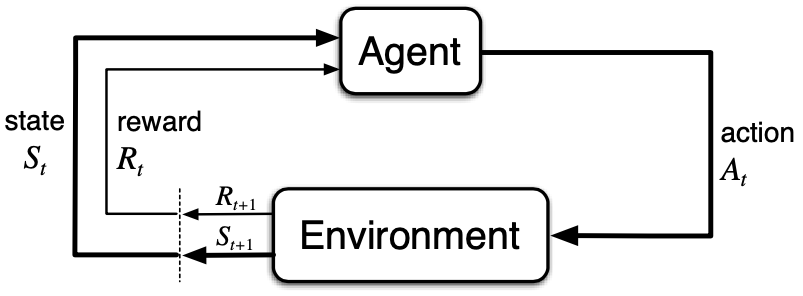
\includegraphics[width=6cm]{rl-loop.png}
		\caption{Typical RL scenario. \cite{10.5555/3312046}}
		\label{fig:rl-loop}
	\end{figure}
	
	\columnbreak

	\begin{itemize}
		\item At each step $t$ the agent:
		\begin{itemize}
			\item Executes action $A_t$
			\item Receives observation $O_t$
			\item Receives scalar reward $R_t$
		\end{itemize}
	
		\item The environment:
		\begin{itemize}
			\item Receives action $A_t$
			\item Emits observation $O_{t+1}$
			\item Emits scalar reward $R_{t+1}$
		\end{itemize}
	\end{itemize}

\end{multicols}


\end{frame}

%------------------------------------------------


\begin{frame}
\frametitle{States and observations}

\begin{itemize}

\item A \textbf{state} $s$ is a complete description of the state of the world
\item An \textbf{observation} $o$ is a partial description of a state
\item Markov decision processes are a mathematical way to describe RL problems

\end{itemize}

\begin{definition}
	A \textbf{MDP} is a tuple $(S,A, P, R, \gamma)$, where:
	\begin{itemize}
		\item $S$ is a (finite) set of Markov states $s \in S$
		\item $A$ is a (finite) set of actions $a \in A$
		\item $P$ is dynamics/transition model for each action, that specifies
		\begin{equation}
			P(s_{t+1} =s'|s_t =s,a_t =a)	
		\end{equation}
		\item $R$ is a reward function
		\begin{equation}
			R(s_t =s,a_t =a)=\E[r_t|s_t =s,a_t =a]	
		\end{equation}
		
		\item $\gamma$ is a discount factor $\gamma \in [0,1]$
	\end{itemize}
\end{definition}

\end{frame}

%------------------------------------------------



\begin{frame}
	\frametitle{Action spaces}
	\begin{itemize}
		\item Different environments allow different kinds of actions
		\item The set of all valid actions in a given environment is called the \textbf{action space}
		\item Depending on the environment, the action spaces could be \textbf{discrete} or \textbf{continuous}
	\end{itemize}
\end{frame}

%------------------------------------------------


\begin{frame}
	
	\frametitle{Policies}
\begin{itemize}
	\item A \textbf{policy} defines the learning agent's way of behaving, it is a mapping from perceived states of the environment (i.e. observations) to actions to be taken when in those states
	\item A policy fully defines the behavior of an agent
\end{itemize}

\begin{definition}
	 A \textbf{policy} $\pi$ is a probability distribution over actions given states
	
	\begin{equation}
	\pi(a | s) = \Pprob[A_t=a|S_t=s]
	\end{equation}

\end{definition}

The MDP and agent's policy together give rise to a \textbf{trajectory} $\tau$, which is a sequence of states and actions in the world:
$$\tau = (s_0, a_0, r_0, s_1, a_1, r_1...)$$

\end{frame}

%------------------------------------------------



\begin{frame}

	\frametitle{Reward and return}
	\begin{itemize}
		\item The reward function $R$ depends on the current state of the world and action just taken:
		$$r_t = R(s_t, a_t)$$
		\item The agent aim to maximize the cumulative reward over a trajectory
		\item The sum of all rewards obtained by the agent is discounted by how far off in the future they are obtained
		\item The discount factor is $\gamma \in [0,1]$
		\item The cumulative reward over a trajectory is:		
			\begin{equation}
			R(\tau) = \sum_{t=0}^{H-1} \gamma^t r_t
			\end{equation}
	\end{itemize}
	
\end{frame}


%------------------------------------------------



\begin{frame}

	\frametitle{RL optimization problem}

		\begin{itemize}
			\item The goal in RL is to select a policy which \textbf{maximizes the expected return} when an agent acts according to it

			\item The policy influences the probability distribution over trajectories
			\item The probability of a $T$-step trajectory is:

			\begin{equation}
				P(\tau|\pi) = \rho_0 (s_0) \prod_{t=0}^{T-1} P(s_{t+1} | s_t, a_t) \pi(a_t | s_t)
			\end{equation}
		
		
		\item The expected return, denoted by $J(\pi)$, is then:

			\begin{equation}
			J(\pi) = \E_{\tau\sim \pi}{[R(\tau)]}
			\label{eq:loss}
			\end{equation}

		\item The central optimization problem in RL can then be expressed by:
			\begin{equation}
			\pi^* = \arg \max_{\pi} J(\pi)
			\label{eq:max_loss}
			\end{equation}
				with $\pi^*$ being the optimal policy.
		\end{itemize}
		
\end{frame}

%------------------------------------------------



\begin{frame}

	\frametitle{Value function}

		Crucial aspects of RL are state-value function and action-value function:

		\begin{definition}
			The \textbf{State-Value Function} of a policy, $V^{\pi}(s)$ is the expected return by starting in state $s$ and always acting according to policy $\pi$:
			\begin{equation}
				V^{\pi}(s) = \E_{\tau \sim \pi} [R(\tau)| s_0 = s]
			\end{equation}
		\end{definition}

		\begin{definition}
			The \textbf{Action-Value Function} of a policy, $Q^{\pi}(s,a)$ is the expected return by starting in state $s$ and taking an arbitrary action $a$ (which may not have come from the policy), and then forever after acting according to the policy $\pi$:
			\begin{equation}
					Q^{\pi}(s,a) = \E_{\tau \sim \pi}[R(\tau)| s_0 = s, a_0 = a]	
			\end{equation}
			
		\end{definition}
	
\end{frame}

%------------------------------------------------




\begin{frame}
	\frametitle{Optimal value function and optimal policy }
	Value functions define a partial ordering over policies,
	$\pi \geq \pi'$ if and only if $v_\pi(s) \geq v_{\pi'}(s)$ for all $s \in S$. There is always at least one policy that is better than or equal to all other policies, this is the optimal policy $\pi^*$.

	\begin{definition}
		The \textbf{Optimal State-Value Function}, $V^*(s)$ is the expected return by starting in state $s$ and always acting according to the \textit{optimal} policy in the environment:
		
		\begin{equation}
			V^{*}(s) = \max_\pi \E_{\tau \sim \pi} [R(\tau)| s_0 = s] = \max_\pi V^\pi(s)
		\end{equation}
	\end{definition}

	\begin{definition}
		The \textbf{Optimal Action-Value Function}, $Q^*(s,a)$ is the expected return by starting in state $s$, taking an arbitrary action $a$, and then forever after acting according to the \textit{optimal} policy in the environment:
		
		\begin{equation}
		Q^*(s,a) = \max_{\pi} \E_{\tau \sim \pi}{[R(\tau)| s_0 = s, a_0 = a]} = \max_\pi Q^\pi(s,a)
		\end{equation}
	\end{definition}

\end{frame}


\begin{frame}
	\frametitle{Optimal value function and optimal policy }
	By having $Q^*(s,a)$, it is possible to directly obtain the optimal action $a^*(s)$:

	\begin{equation}
		a^*(s) = \argmax_{a \in A} Q^* (s,a)
	\end{equation}

	Therefore an optimal policy can be found by maximizing over $Q^*(s,a)$:

	\begin{equation}
		\pi^*(a|s) = 
		\begin{cases}
			1 & if \; a = \argmax_{a \in A} Q^*(s,a)\\
			0 & otherwise
		\end{cases}
		\label{eq:opt-policy}
	\end{equation}

\end{frame}

%------------------------------------------------

\section{RL algorithms}


\begin{frame}
	\frametitle{RL algorithms}
	
	\tableofcontents[ 
	currentsubsection, 
	hideothersubsections, 
	sectionstyle=show/shaded,
	]
	
\end{frame}


\begin{frame}
	\frametitle{Taxonomy of RL algorithms}
	The final objective of RL is to find the best policy, i.e.:

	\begin{equation}
		\pi^* = \argmax_\pi \E_{\tau \sim \pi}{[R(\tau)]}
		\label{eq:objective}
	\end{equation}
	

	There are a variety of algorithms to do so, depending on what to learn and how to learn it.

	\begin{figure}[h]
		\centering
		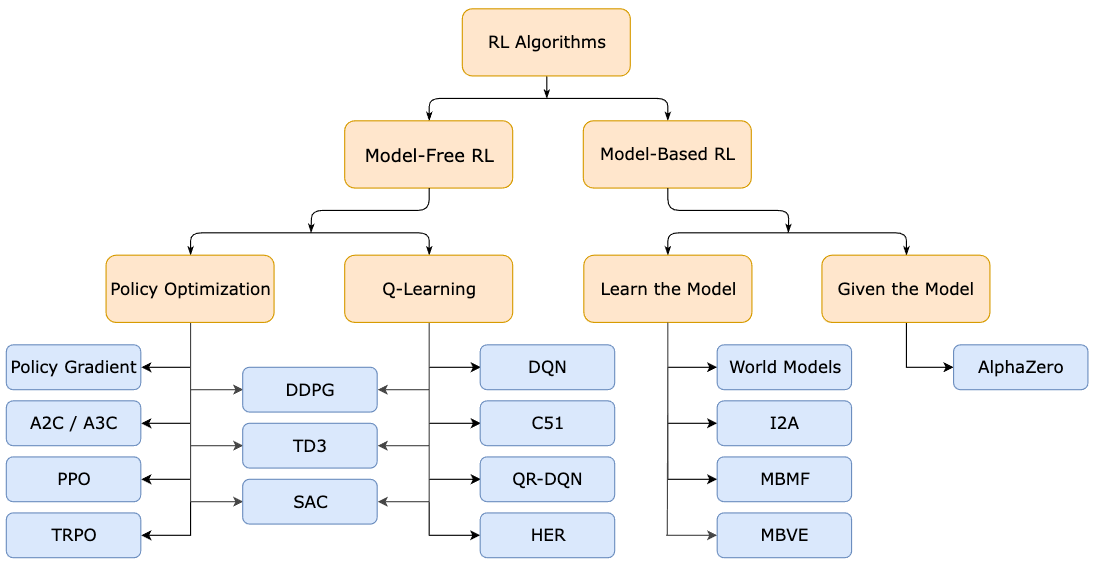
\includegraphics[width=7cm]{rl-taxonomy.png}
		\caption{A non-exhaustive taxonomy of RL algorithms.\cite{SpinningUp2018}}
		\label{fig:rl-taxonomy}
	\end{figure}

\end{frame}


\begin{frame}
	\frametitle{Q-Learing}
	An example of RL algorithm is Q-learning:

	\begin{itemize}
		\item Q-Learning methods learn an approximation $Q_{\theta}(s,a)$ for the optimal action-value function, $Q^*(s,a)$
		\item The Q-learning algorithm keeps an estimate $Q(s,a)$ of $Q^*(s,a)$ for each state-action pair $(s,a) \in S \times A$
		\item By observing $(s_t, a_t, r_{t+1}, s_{t+1})$ the estimates are updated
	\end{itemize}
	
	The idea behind Deep Reinforcement Learning is that since Q-Learning is simply function approximation, a Deep Neural Network could be used to approximate this function. 

\end{frame}

%------------------------------------------------

\section{Case study: AlphaGo Zero}

\begin{frame}
	\frametitle{AlphaGo Zero}
	
	\tableofcontents[ 
	currentsubsection, 
	hideothersubsections, 
	sectionstyle=show/shaded,
	]
	
\end{frame}


\begin{frame}
	\frametitle{Motivation of AlphaGo Zero}
	\begin{itemize}
		\item The game of Go is one of the most challenging games for artificial intelligence
		\begin{itemize}
			\item Enormous search space and the difficulty of evaluating board positions and moves
		\end{itemize}
		\item Search algorithms that use minimax, alpha-beta pruning and evaluation function can not be used in the game of Go due to its huge complexity.
		\begin{itemize}
			\item This techniques were used in DeepBlue\cite{CAMPBELL200257} to beat Garry Kasparov in the game of chess
		\end{itemize}
		
	\end{itemize}
	
	\begin{table}

		\tiny
		\centering

		\caption{Complexity of the most famous board games.}
		
		\begin{tabular}{lccccc}

		\hline
		\textbf{Game}  &
		Board size (positions)  &
		Game-tree complexity (log to base 10)  &
		Complexity class\\
		\hline
		\hline
		\textbf{Tic-tac-toe}	& 9  & 5 & PSPACE-complete\cite{Reisch1981HexIP} \\
		\textbf{Connect Four} & 42 & 21 & in PSPACE \cite{Allis1994SearchingFS} \\
		\textbf{Checkers} & 32  & 40   & EXPTIME-complete \cite{Robson1984NBN} \\
		\textbf{Chess} & 64 & 123  & EXPTIME-complete \cite{FRAENKEL1981199} \\
		\textbf{Go (19x19)} & 361 & 360 & EXPTIME-complete \cite{inproceedings} \\
		\hline
		\end{tabular}
		\label{tab:game-complexity}
		
	\end{table}

	
	\begin{figure}[h]
		\centering
		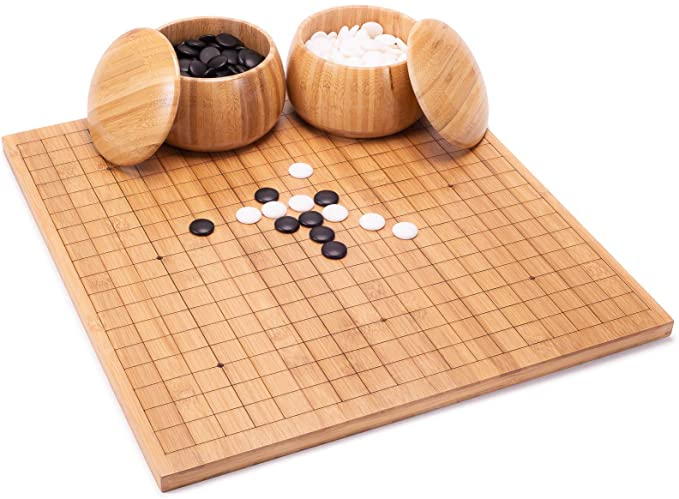
\includegraphics[width=2cm]{go-board.jpg}
	\end{figure}

\end{frame}

%------------------------------------------------

\begin{frame}
	\frametitle{AlphaGo Zero}
	Characteristics of AlphaGo Zero:
	\begin{itemize}
		\item AlphaGo Zero \cite{silver2017mastering}, is an algorithm based on reinforcement learning
		\item It started from zero, without human knowledge beyond game rules
		\item AlphaGo Zero achieved superhuman performance in Go.
	\end{itemize}

	A deep neural network is used for value-function approximation:
	\begin{itemize}
		\item Takes as input the raw board representation $s$
		\item Has two outputs (multitask learning):
		\begin{itemize}		
			\item Vector $p$: the vector of move probabilities $p$ represents the probability of selecting each move, $p_a = P(a | s)$
			\item Scalar $v$: the value $v$ is a scalar evaluation, estimating the probability of the current player winning from position $s$
		\end{itemize}
	\end{itemize}
\end{frame}


%------------------------------------------------

\begin{frame}
	\frametitle{Self-play in AlphaGo Zero}
	
	\begin{itemize}
		\item The neural network in AlphaGo Zero is trained from games of self-play
		\item In each position $s$, a MCTS search is executed, guided by the neural network $f_\theta$
		
		\item The MCTS select much stronger moves than the raw move probabilities $p$ of the neural network $f_\theta(s)$

		\begin{itemize}
			\item MCTS can then be viewed as a policy improvement operator
		\end{itemize}
		
		\item During the self-play the MCTS-based policy is used to select each move, and the game winner $z$ is used as a sample of the value $v$ (the winning player)
		\item Parameters are updated to make the move probabilities and value $f_\theta(s) = (p, v) $ match the search probabilities and self play winner $(\pi, z)$.
	\end{itemize}
\end{frame}


\begin{frame}
	\frametitle{Self-play in AlphaGo Zero}
		
	\begin{figure}[H]
		\centering
		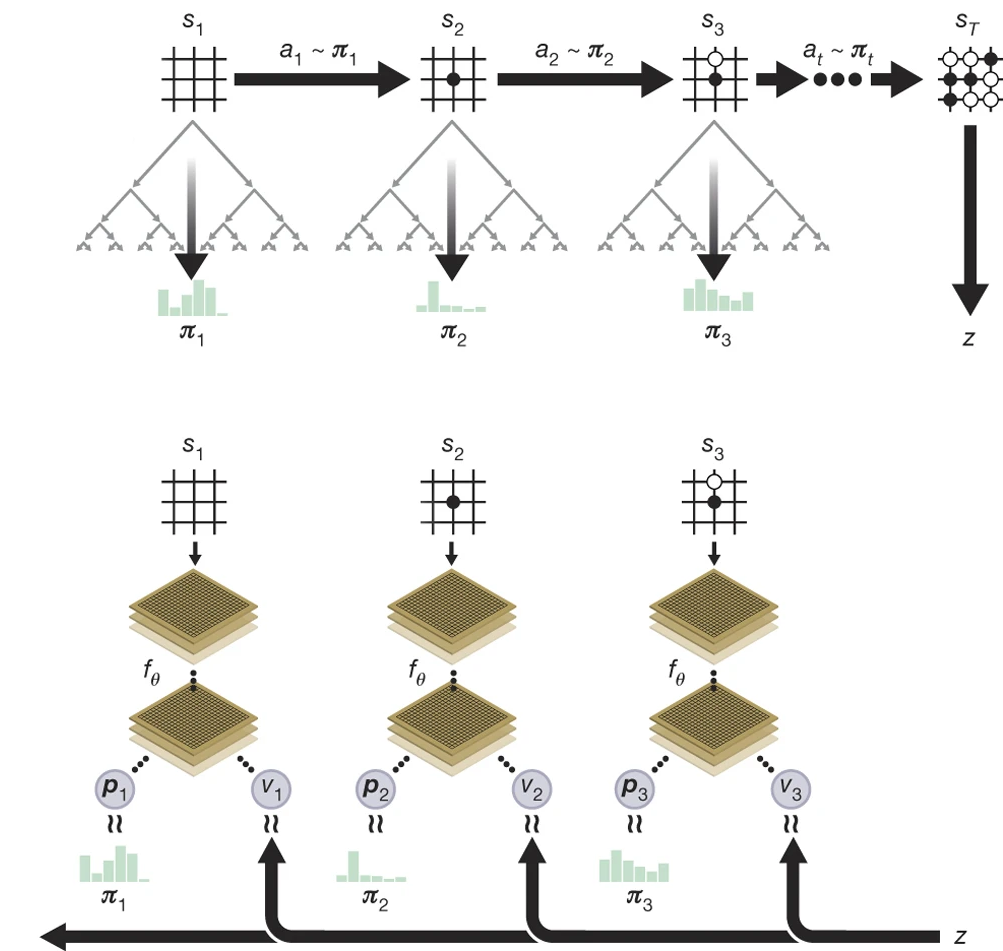
\includegraphics[width=4cm]{alpha_go_zero_training.png}
		
		\caption{
			\textbf{Self-play} and \textbf{training} AlphaGo Zero.\cite{Silver_2016}
			}
		\label{fig:alpha-zero-self_play}
	\end{figure}
	
	The parameters $\theta$ are adjusted by gradient descent on the loss function $L$:

	\begin{equation}
		f_\theta(s) = (p,v),\quad L = (z-v)^2 - \pi_t log(p) + c \norm{\theta}^2
	\end{equation}
\end{frame}


\begin{frame}
	\frametitle{MCTS in AlphaGo Zero}
	\begin{itemize}
	\item The MCTS uses the neural network $f_\theta$ to guide its simulations.
	$$f_\theta(s) = (P(s, \cdot), \, V(s))$$
		
	
	\item Each simulation starts from the root state and selects moves:
	\begin{equation}
		a_t  = \argmax_a{Q(s_t,a) + U(s_t,a)}
	\end{equation}

	\begin{equation}
		Q(s, a) = \frac{1}{N(s,a)} \sum_{s'\, | \, s,\, a \rightarrow s'}{V(s')},
	\end{equation}

	\begin{equation}
		U(s, a) = c_{puct}P(s, a)\frac{\sum_b N(s,b)}{1+N(s,a)}
	\end{equation}

	\item $U(s_t,a)$ acts as an exploration factor governed by $c_{puct}$
	\begin{itemize}
		\item This strategy initially prefers actions with high prior probability and low visit count, but asymptotically prefers actions with high action value.
	\end{itemize}
	\end{itemize}
\end{frame}


\begin{frame}
	\frametitle{Empirical results of AlphaGo Zero}
	
	\begin{figure}[H]
		\centering
		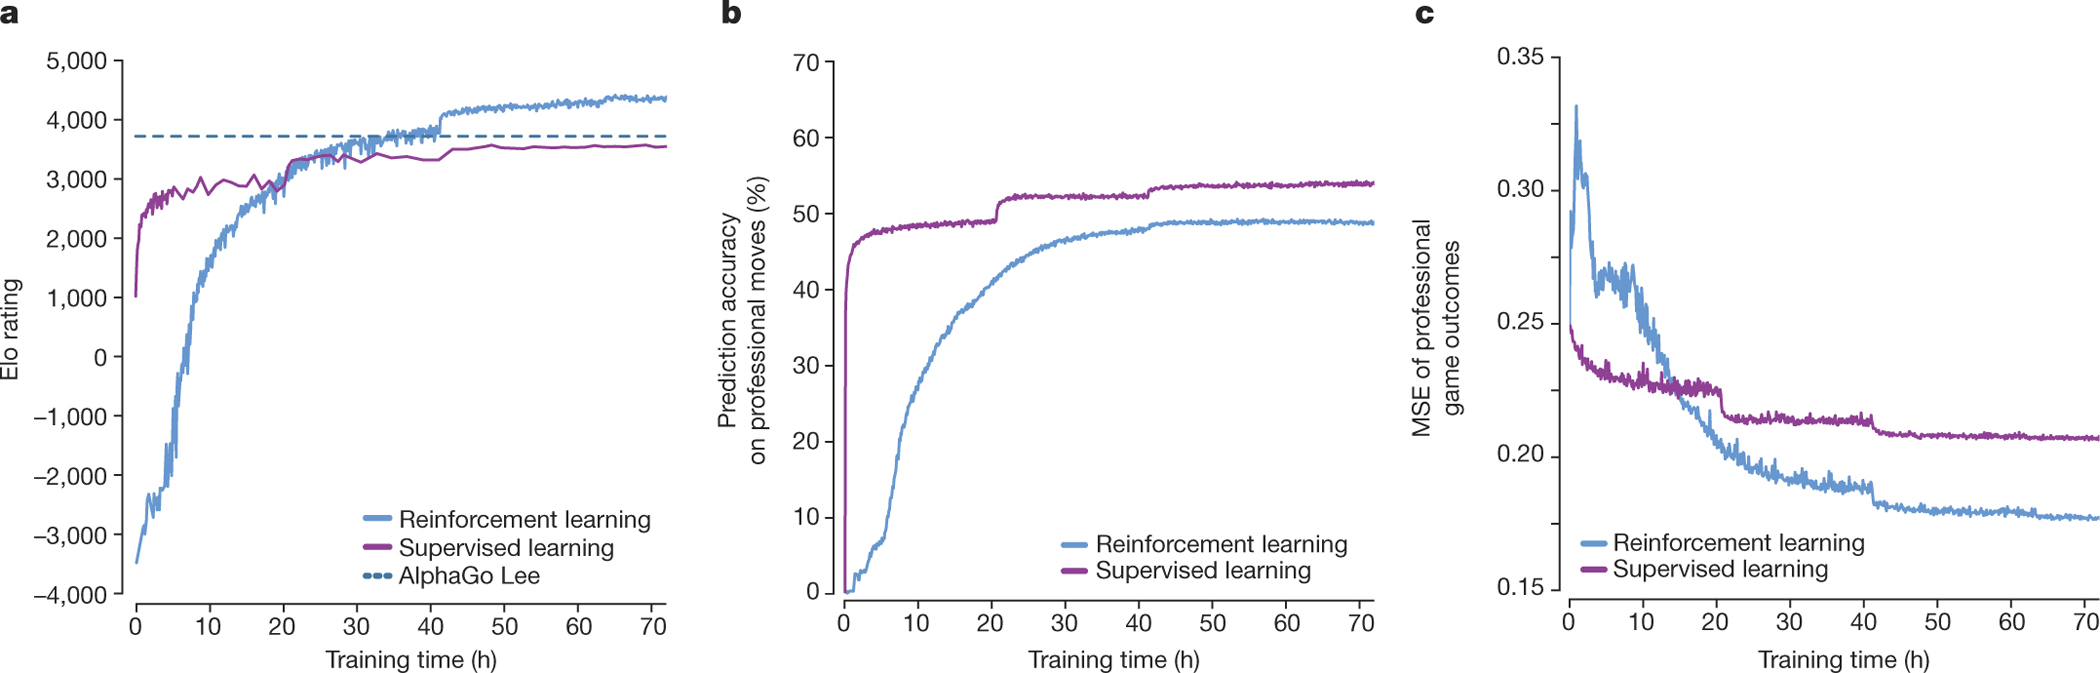
\includegraphics[width=11cm,trim={0px 0px 0px 45px},clip]{alpha-go-zero_empirical_results.png}
		\caption{AlphaGo Zero performance. \cite{Silver_2016}}
	\end{figure}

	\begin{itemize}
		\item AlphaGo zero performs worse in predicting master Go player moves
		\item It is better in predicting the actual outcome of a game (lower MSE)
		\item There is no a ceiling to the performances imposed by the human knowledge.
	\end{itemize}

\end{frame}


\section{Hands-on: Connect4 Zero}

\begin{frame}
	\frametitle{Hands-on: Connect4 Zero}
	
	\tableofcontents[ 
	currentsubsection, 
	hideothersubsections, 
	sectionstyle=show/shaded,
	]
	
\end{frame}

\begin{frame}
	\frametitle{Connect4 Zero}

	\begin{itemize}
		\item Use the techniques of AlphaGo Zero \cite{silver2017mastering} to achieve master level in Connect4
		\item I considered the game of Connect4 due to the limited computational resources at my disposal
		\item Starting from this code\footnote{\url{https://github.com/suragnair/alpha-zero-general}} the support of Connect4 has been added.\footnote{\url{https://github.com/gianlucagiudice/alpha-zero-general}}  Also I added:
		\begin{itemize}
			\item A graphical user interface to play against the agent
			\item A simpler neural network architecture
			\item Episodes of self-play are performed in parallel to drastically reduce the training time (taking inspiration form the work of David Silver "Playing Atari with Deep Reinforcement Learning" \cite{mnih2013atari})

		\end{itemize}

	\end{itemize}

\end{frame}

%------------------------------------------------

\begin{frame}
	\frametitle{Connect4 Zero}
	\Huge{\centerline{Live Demo}}
\end{frame}

%------------------------------------------------

\section{}
\begin{frame}
	\frametitle{Connect4 Zero}
	\Huge{\centerline{Thank you for your attention!}}
\end{frame}

%------------------------------------------------

\section{}
\begin{frame}[allowframebreaks]
	\frametitle{Refenreces}
	\printbibliography
\end{frame}

%------------------------------------------------

\end{document} 